\section{Auswertung}
\label{sec:Auswertung}
Sämtliche im Folgenden durchgeführten Ausgleichsrechnungen werden mit der \emph{curve fit} Funktion aus dem für \emph{Python} geschriebenen package \emph{NumPy}\cite{scipy} durchgeführt. Fehlerrechnungen werden mit dem für \emph{Python} geschriebenen package \emph{Uncertainties}\cite{uncertainties} ausgeführt.

Die Auswertung der verschiedenen Messungen folgt in der Reihenfolge wie sie auch aufgenommen wurden (siehe \cite{skript}). Einige der Datensätze wurde von der System-Software \emph{EASy} in dem Format \emph{.h5} gespeichert. Mit einem vom Praktikumsbetreuer zur Verfügung gestellten Python-Skript, wurde eine Vorauswertung durchgeführt und die für die Auswertung relevanten Daten in dem Format \emph{.txt} gespeichert.

\subsection{Strom-Spannungs-Kennlinie}
\label(sec:IV)
In Abbildung \ref{fig:IV} ist die IV-Kurve des Silizium-Streifen-Sensors dargestellt. Bei kleinen Spannung ist ein Anstieg des Leckstroms zu beobachten, gefolgt von einem Plateau. Der Übergang in dieses Plateau ist bei $V=\SI{70}{\volt}$ erreicht. Aus diesem Grund wird dieser Wert als Abschätzung für die Depletionsspannung $U_{dep}$ verwendet.

\begin{figure}[H]
  \centering
  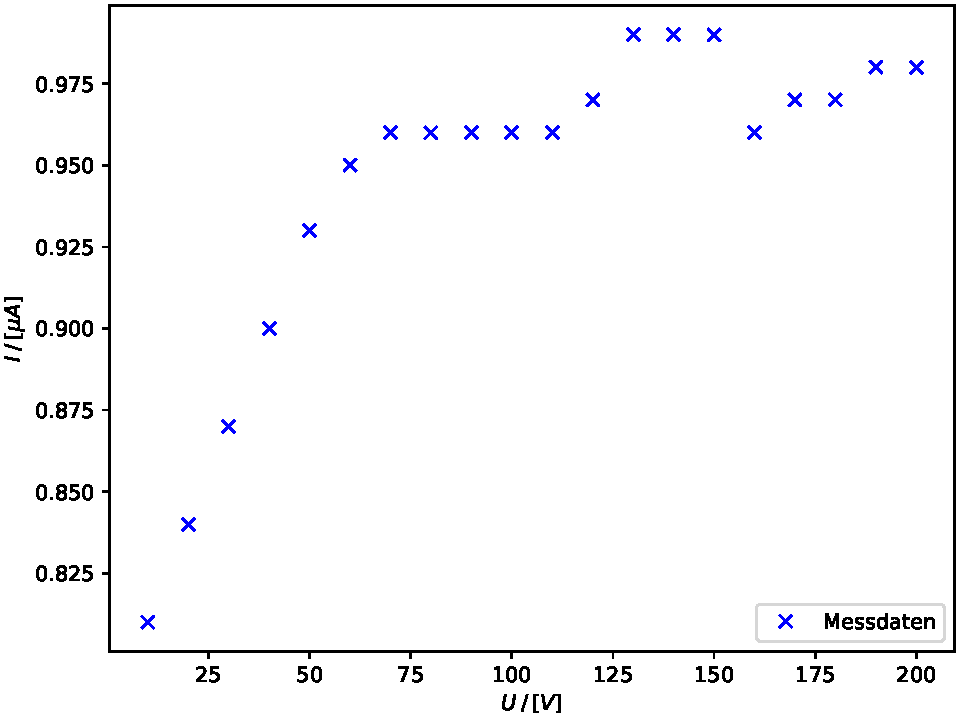
\includegraphics{build/IV_Kurve.pdf}
  \caption{Messung des Leckstroms in Abhängigkeit der Spannung.}
  \label{fig:IV}
\end{figure}

\subsection{Pedestal und Noise}
Für eine Übersicht sind in Abbildung \ref{fig:ADC} die ADC-Counts in Abhängigkeit der Events und der Channel dargestellt. In dieser Darstellung sind die ADC-Counts ein Maß für das Grundrauschen ohne Signal. 

\begin{figure}[H]
  \centering
  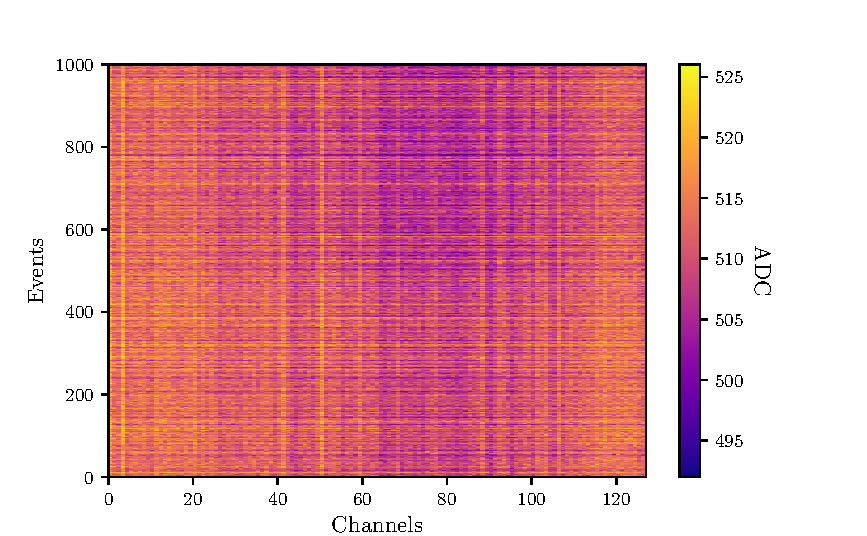
\includegraphics{build/ADC.pdf}
  \caption{ADC-Counts in Abhängigkeit der Events und der Channel.}
  \label{fig:ADC}
\end{figure}


Es zeigt sich, dass die Channel im Intervall [65,90] ein geringes Rauschen als an den Rändern des Sensors aufweisen. Aus diesem Datensatz wird nach Gleichung XXX das Pedestal und nach Gleichung XXX der Common-Mode-Shift bestimmt. Da nach \cite{skript} der Common-Mode-Shift um 0 Gaußverteilt ist, werden die Messwerte in Bins der Länge 0.25 unterteilt. In Abbildung \ref{fig:pedestals} sind die Pedestals und in \ref{fig:CMS} der Common-Mode-Shift dargestellt. 

\begin{figure}[H]
  \centering
  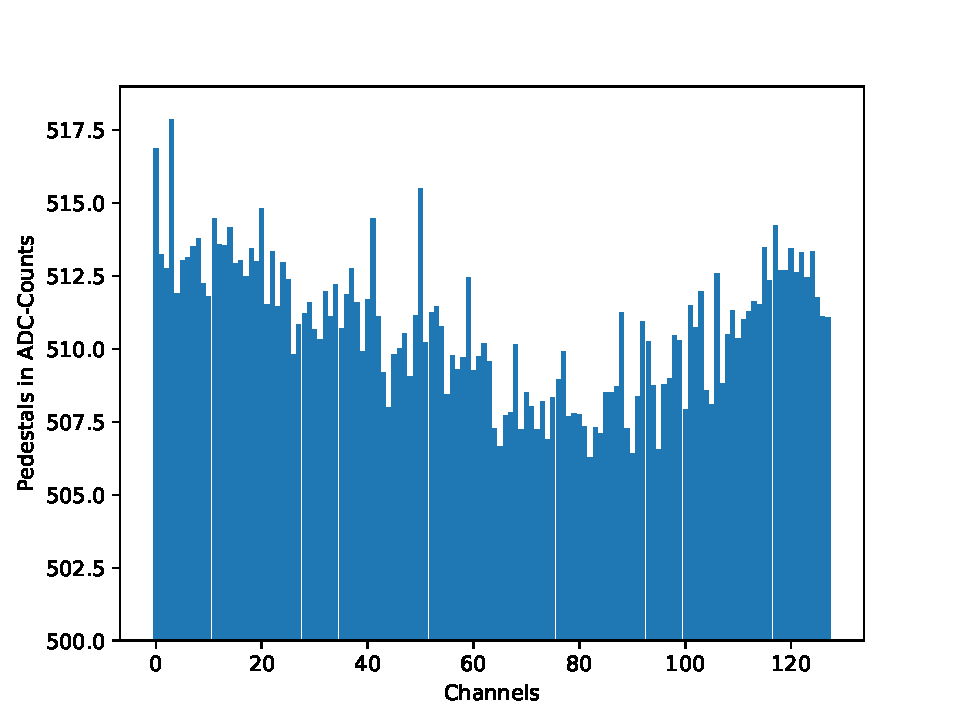
\includegraphics{build/Pedestals.pdf}
  \caption{Pedestals.}
  \label{fig:pedestals}
\end{figure}

 
\begin{figure}[H]
  \centering
  \includegraphics{build/CMS_Gauß.pdf}
  \caption{Common-Mode-Shift.}
  \label{fig:CMS}
\end{figure}

Aus den zuvor beschriebenen Größen wird unter Verwendung von Gleichung XXX die Noise bestimmt, in Abbildung \ref{fig:noise} ist diese dargestellt.

\begin{figure}[H]
  \centering
  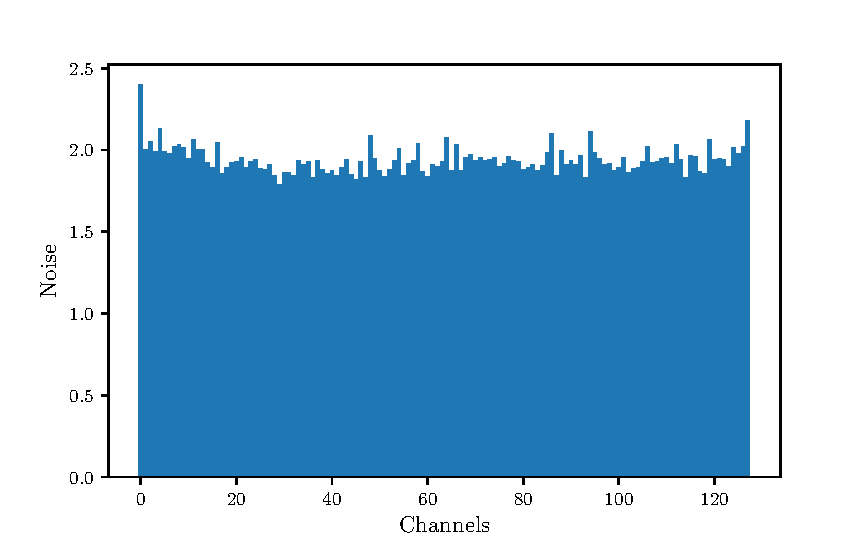
\includegraphics{build/Noise.pdf}
  \caption{Noise.}
  \label{fig:noise}
\end{figure}

\subsection{Kalibrationsmessung}

Für fünf verschiedene Channel ist eine Kalibrationsmessung mit einem definierten Signal vorgenommen worden. In Abbildung \ref{fig:calib} sind die Messwerte für alle fünf Channel bei $\SI{90}{\volt}$ und für Channel 10 bei $\SI{0}{\volt}$ aufgetragen. Zusätzlich ist in Abbildung \ref{fig:calib_detail} eine Detailansicht dargestellt.

\begin{figure}[H]
\centering
\begin{subfigure}{.5\textwidth}
	\centering
	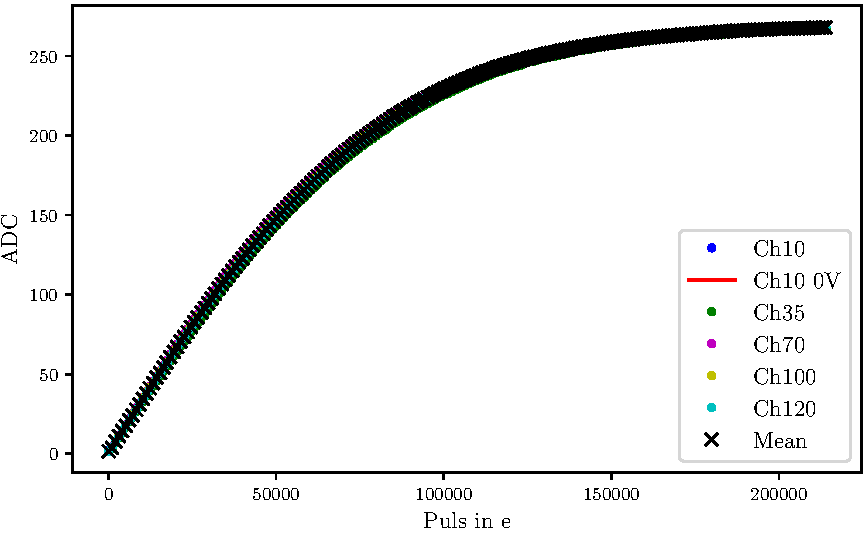
\includegraphics[width=0.95\textwidth]{build/Calib.pdf}
	\caption{}
	\label{fig:calib}
\end{subfigure}%
\begin{subfigure}{.5\textwidth}
	\centering
	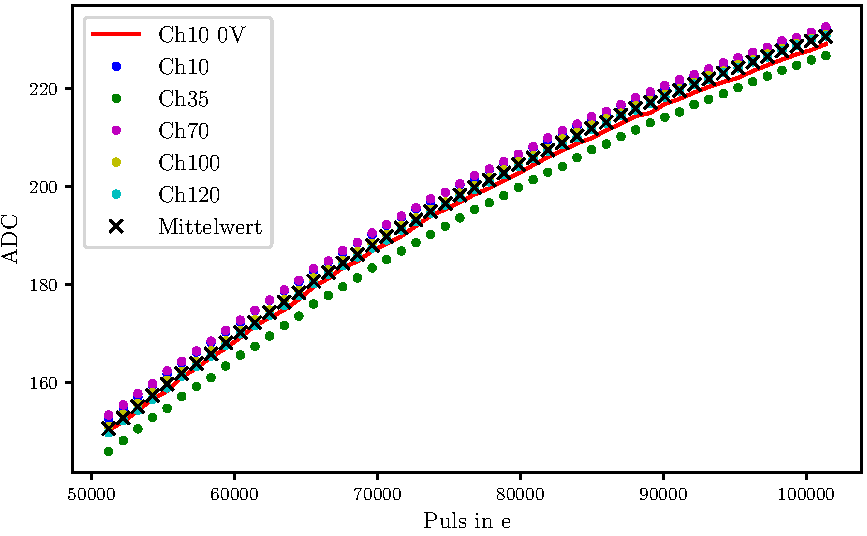
\includegraphics[width=0.95\textwidth]{build/Calib_detail.pdf}
	\caption{}
	\label{fig:calib_detail}
\end{subfigure}
\caption{Zusammenhang zwischen dem Signal (ADC) und den Pulsen.}
\label{fig:calib}
\end{figure}

Um in späteren Kapitel die Signale in Pulse umrechnen zu können wird mit Hilfe eines Polynoms vierter Ordnung ein mathematischer Zusammenhang zwischen diesen beiden Größen gesucht.
Die verwendende Fitfunktion lautet:
\begin{align}
	Puls(ADC)=a \cdot ADC^4 + b \cdot ADC^3 + c \cdot ADC^2 + d \cdot ADC + e 
\end{align} 
Unter Verwendung dieser Funktion fällt in Abbildung \ref{fig:calib_fit} auf, dass für den fast linearen Anstieg bei kleinen Signalen die Koeffizienten der Therme höherer Ordnung relativ klein sein müssen, jedoch um den annähernd exponentiellen Anstieg beschreiben zu können, werden große Koeffizienten vor den höheren Ordnung benötigt. Da dies einen Widerspruch dargestellt, wird die Ausgleichsfunktion nur mit den Daten im Intervall [0,250] bestimmt. In Abbildung XXX wird diese Grenze graphisch deutlich gemacht, ab der die Ausgleichsrechnung eine große Abweichung zu dem Verlauf der Messwerte aufzeigt.

\begin{figure}[H]
  \centering
  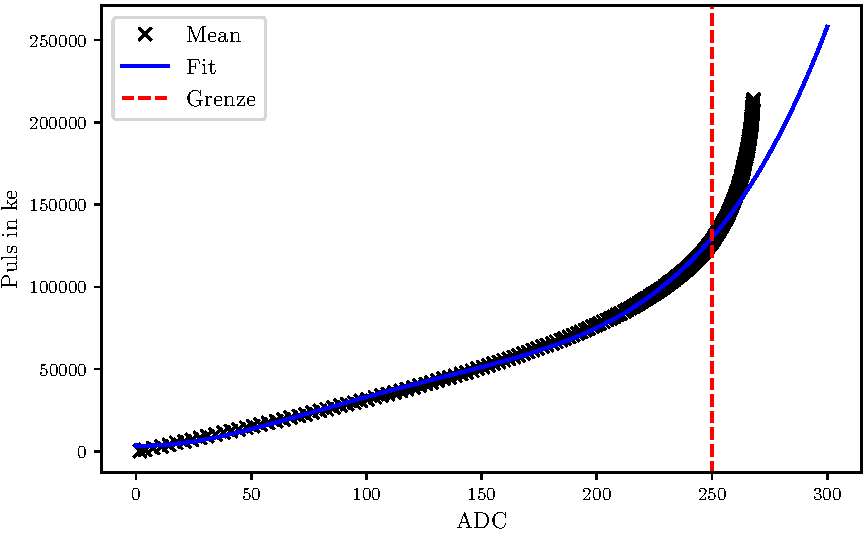
\includegraphics{build/Calib_fit.pdf}
  \caption{Ausgleichsrechnung mit den Messdaten im Intervall [0,250].}
  \label{fig:calib_fit}
\end{figure}

\subsection{Vermessung der Streifensensoren mittels des Lasers}

Wie in Kapitel XXX beschrieben, werden der Sensor mittels Laser vermessen. Die Messdaten sind in Abbildung \ref{fig:laserscan_komplett} für den kompletten Sensor und in \ref{fig:laserscan_zoom} für die betroffenen Streifen dargestellt. 

\begin{figure}[H]
\centering
\begin{subfigure}{.5\textwidth}
	\centering
	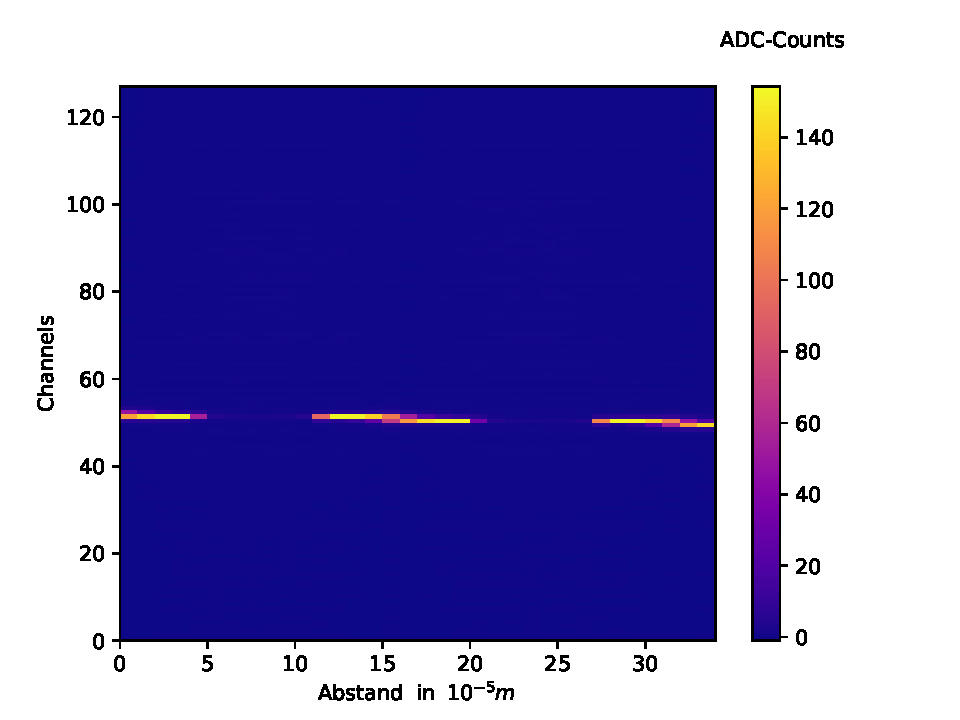
\includegraphics[width=1.05\textwidth]{build/Laserscan_komplett.pdf}
	\caption{}
	\label{fig:laserscan_komplett}
\end{subfigure}%
\begin{subfigure}{.5\textwidth}
	\centering
	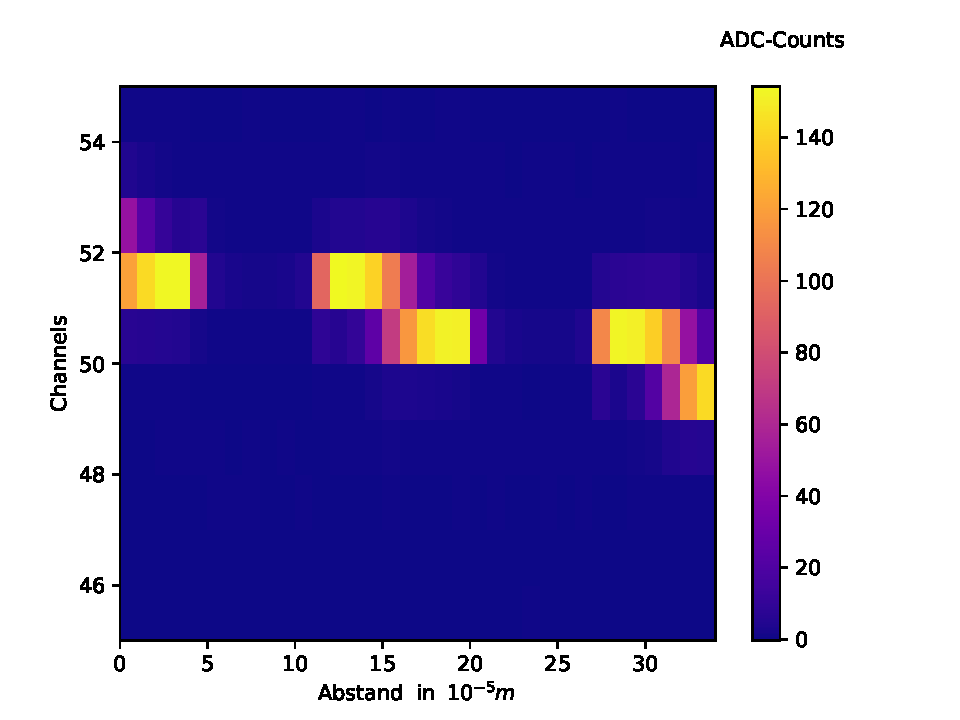
\includegraphics[width=1.05\textwidth]{build/Laserscan_zoom.pdf}
	\caption{}
	\label{fig:laserscan_zoom}
\end{subfigure}
\caption{Signal (ADC) in Abhängkeit des Position auf dem Sensor und des Channels.}
\label{fig:ladserscan}
\end{figure}

Für die Abschätzung der Streifenbreite, des Abstands der Streifen und der Größe des Laserspots, ist in Abbildung \ref{fig:laserscan_pos} für die Channel 50, 51 und 52 das Signal (ADC) gegen den Abstand aufgetragen.

\begin{figure}[H]
  \centering
  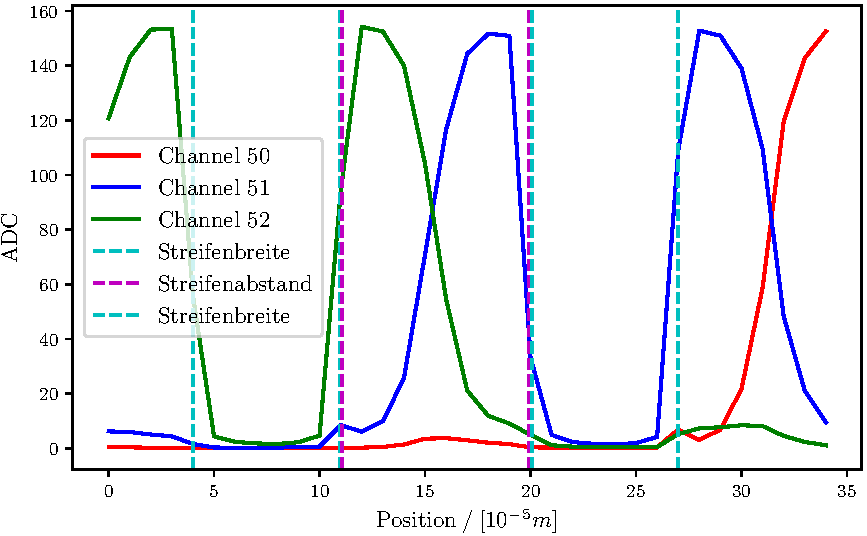
\includegraphics{build/Laserscan_Pos.pdf}
  \caption{Darstellung des Signals der Channel 50, 51 und 52.}
  \label{fig:laserscan_pos}
\end{figure}

Der plötzliche Einbruch des Signals lässt darauf schließen, dass der Laser sich über einem Streifen befindet, da das Aluminium den Strahl komplett reflektiert. Maximal wird das Signal, wenn der Laserspot sich exakt neben dem Streifen und der Hälfte des Abstand der Streifen untereinander befindet (siehe Abbildung \ref{fig:laserscan_pos} , z.B. bei Abstand \SI{120}{\micro\meter}). Genau zwischen den Streifen wird das durch den Laser verursachte Signal zwischen den beiden nächsten Streifen aufgeteilt (siehe Abbildung \ref{fig:laserscan_pos}, z.B. bei Abstand \SI{150}{\micro\meter}). Die Spotgröße des Lasers kann abgeschätzt werden, indem der Abstand zwischen den Positionen vermessen wird, bei denen das Signal wieder beginnt anzusteigen und bei dem es maximal ist. Mit Hilfe von Abbildung \ref{fig:laserscan_pos} können die Größen nun wie folgt abgeschätzt werden:
\begin{align}
	\text{Breite} &= \SI{70}{\micro\meter}\\
	\text{Abstand} &= \SI{90}{\micro\meter}\\
	\text{Spotdurchmesser} &= \SI{20}{\micro\meter}
\end{align}

\subsection{Charge Collection Efficiency des Lasers}
label{sec:CCE}
In Abbildung \ref{fig:CEE_fit} ist die Effizienz des Sensors gegen die Spannung aufgetragen. Da für diese Messung der Laserspot neben Channel 50 platziert worden ist, ist das Sigal in diesem Channel maxmimal und wir deshalb zur Bestimmung der Charge Collection Efficiency (CCE) verwendet. 

Ebenfalls wie die IV-Kurve aus Kapitel \ref(sec:IV), geht die CCE ab der Depletionsspannung in ein Plateau über. Da ab dieser Spannung sich die Größe der Depletionszone nicht mehr verändert, kann auch die Effizienz nicht mehr steigen. Mit Hilfe von Gleichung XXX und unter Berücksichtigung von Gleichung XXX ergibt sich die in Abbildung \ref{fig:CEE_fit} die eingezeichnete Ausgleichsrechnung. 

\begin{figure}[H]
  \centering
  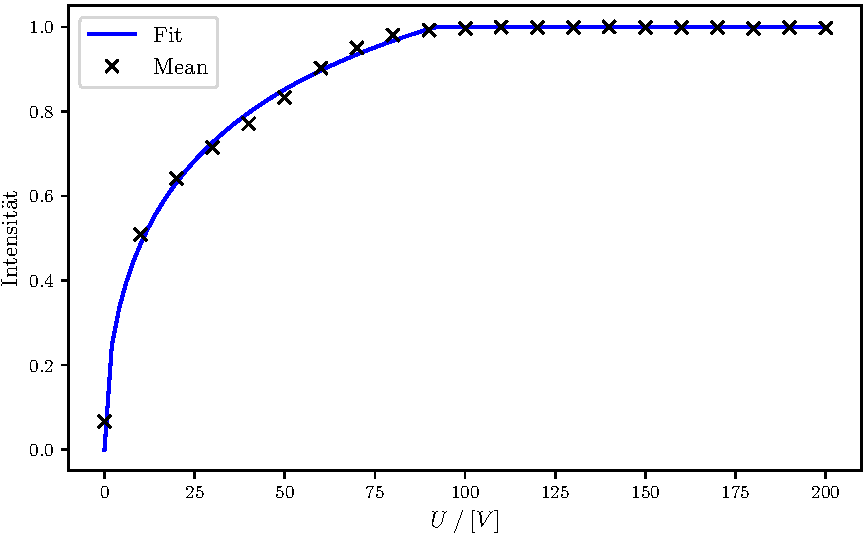
\includegraphics{build/CCE_fit.pdf}
  \caption{Charge Collection Efficiency für Channel 50 in Abhängigkeit der Spannung.}
  \label{fig:CEE_fit}
\end{figure}

Die Fitparameter lauten:

\begin{align}
  U_{dep} &= \SI{92+-5}{\volt}
 \\
  a &= \SI{221+-24}{\micro\meter}
 
\end{align}

\subsection{Charge Collection Efficiency der Sr-Quelle}
Für eine analoge Darstellung zu Abbildung \ref{fig:CEE_fit} ist in Abbildung \ref{fig:CEEQ_fit} die normierte mittlere CCE der $\beta$-Quelle gegen die Spannung aufgetragen. Auch hier ist wieder bei höheren Spannung die Ausbildung eines Plateaus zu beobachten.

\begin{figure}[H]
  \centering
  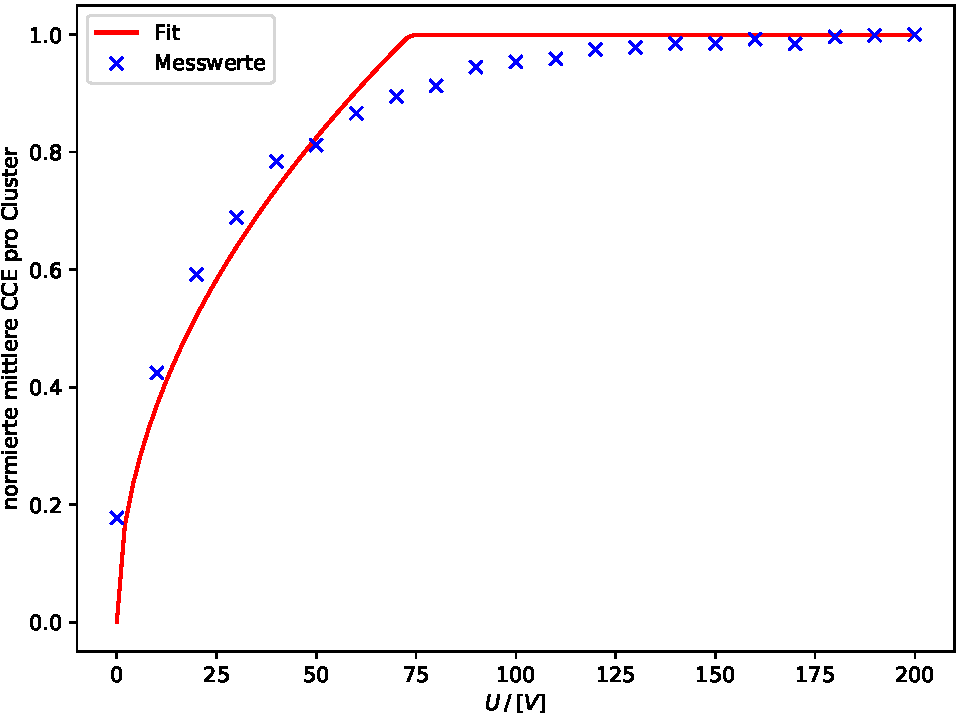
\includegraphics{build/CCEQ_fit.pdf}
  \caption{Charge Collection Efficiency der $\beta$-Quelle in Abhängigkeit der Spannung.}
  \label{fig:CEEQ_fit}
\end{figure}

Mit der selben Ausgleichsrechnung wie in Kapitel \ref{sec:CCE} ergibt sich die Depletionsspannung $U_{dep} = \SI{74+-4}{\volt}
$.

\subsection{Großer Quellenscan}
Für den großen Quellenscan, bei dem 1000000 Events abgewartet werden, wird in Abbildung \ref{fig:frequency_channel} die normierte Häufigkeit der Anzahl der Channel pro Event und in Abbildung \ref{fig:frequency_cluster} die normierte Häufigkeit der Anzahl der Cluster pro Event dargestellt. 

\begin{figure}[H]
\centering
\begin{subfigure}{.5\textwidth}
	\centering
	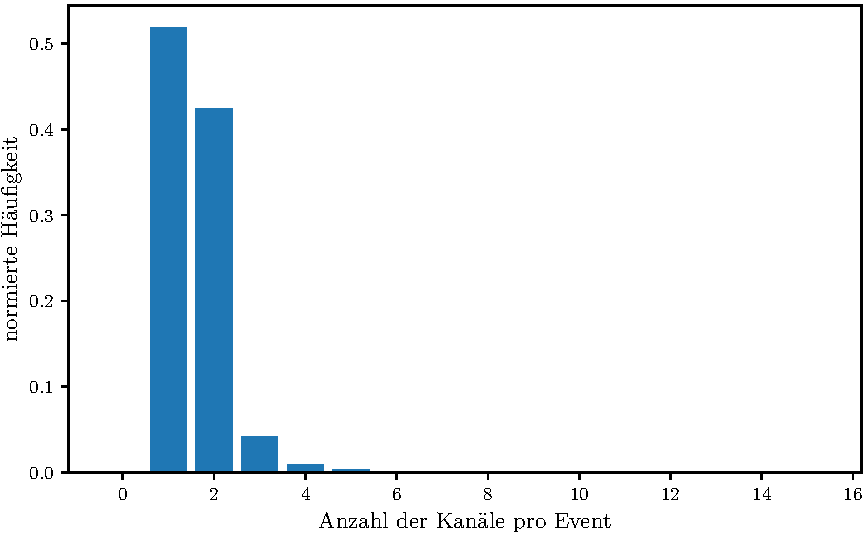
\includegraphics[width=0.9\textwidth]{build/Quellenmessung_frequeny_channel.pdf}
	\caption{}
	\label{fig:frequency_channel}
\end{subfigure}%
\begin{subfigure}{.5\textwidth}
	\centering
	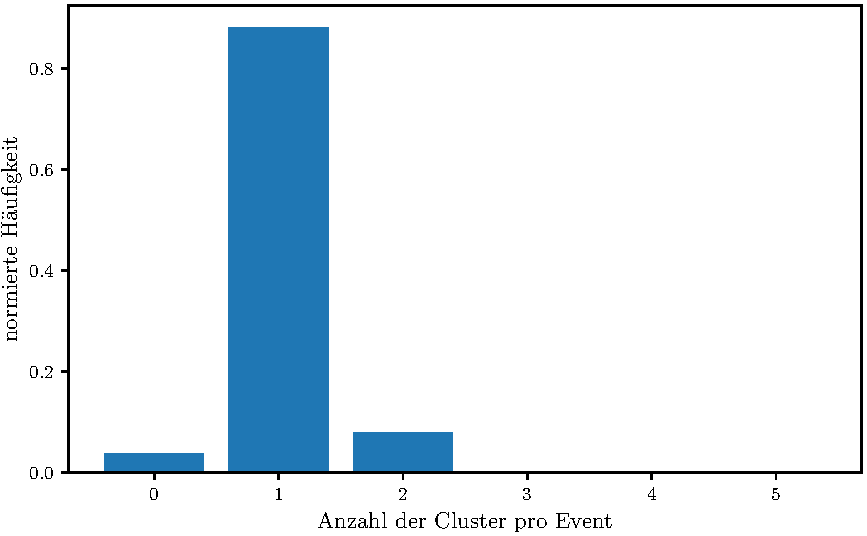
\includegraphics[width=0.9\textwidth]{build/Quellenmessung_frequeny_cluster.pdf}
	\caption{}
	\label{fig:frequency_cluster}
\end{subfigure}
\caption{Normierte Häufigkeit der Channel bzw. Cluster pro Event. Es sind nur die Channel bzw. Claster dargestellt, die einen Eintrag ungleich Null aufweisen.}
\label{fig:großer_quellenscan_1}
\end{figure}

Aus den Abbildung folgt, dass im wesentlichen nur ein bis zwei Streifen, also Channel, ein einzelnes Event registrieren. Des weiteren bildet sich in den meisten Fällen nur ein Cluster pro Event. In Abbildung \ref{fig:CEE_fit} ist die normierte Trefferrate eines Channels über den Zeitraum von 1Mio. Events dargestellt.


\begin{figure}[H]
  \centering
  \includegraphics{build/Quellenmessung_Hitmap.pdf}
  \caption{Trefferrate pro Channel.}
  \label{fig:CEE_fit}
\end{figure}

Es ist zu erkennen, dass die Probe mittig über dem Sensor positioniert worden ist, da sich das Maximum bei etwa Channelnummer 65 ausbildet. Die Streifen am Rand des Sensor weisen jedoch auf kein gaußartiges verhalten hin, sondern steigen wieder und könnten eventuell auf lange Sicht eine Plateau bilden. Da die Differenz zwischen Maximum und Hit an den Rändern sich nur um einen Faktor von etwa 0.25 unterscheidet, ist nicht davon auszugehen, dass die Hits am Rand vom Noise überlagert sind.

In Abbildung \ref{fig:energy} ist das Energiespektrum der Quellenmessung dargestellt. 

\begin{figure}[H]
  \centering
  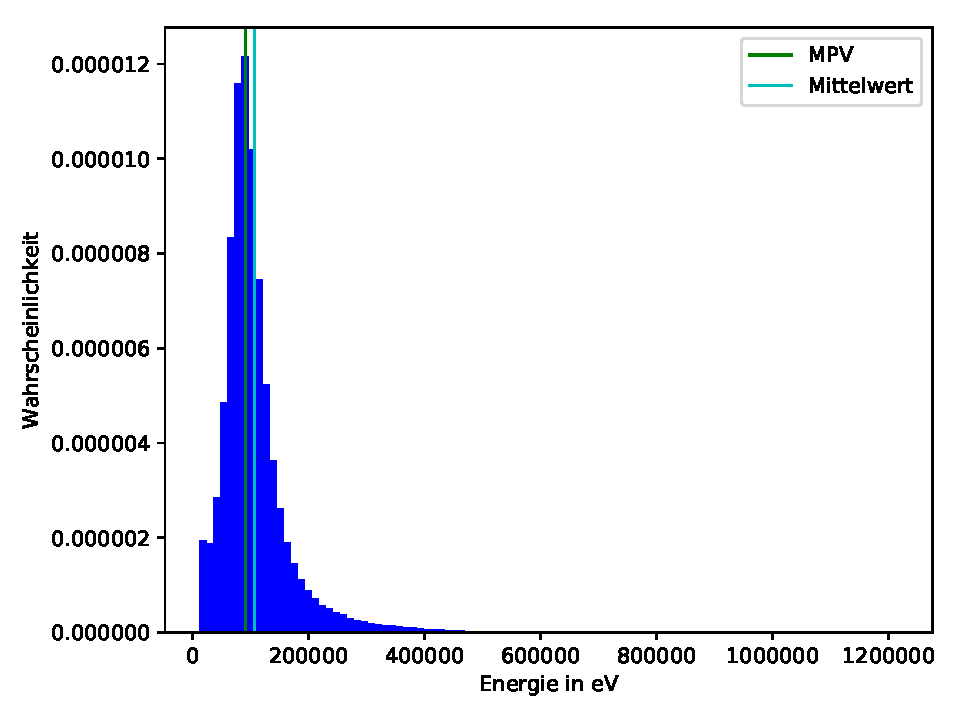
\includegraphics{build/big_clusterenergie_charge.pdf}
  \caption{Energiespektrum unterteilt in 100 Bins.}
  \label{fig:energy}
\end{figure}

Hierfür werden die ACD-Counts mit der Ausgleichsfunktion in Kapitel \ref{sec:CCE} in Pulse umgerechnet. Danach erfolgt die schlussendliche Umrechnung in das Energiespektrum, mit dem Wissen, dass die Erzeugung einen Elektronen-Loch-Paares in Silizium eine Energie von $\SI{3.6}{\eV}$ benötigt. Eingezeichnet sind in der Abbildung die mittlere Energie ($\bar{E}=\SI{108+-62}{\kilo\electronvolt}
$) und die wahrscheinlichste Energie ($MPV=\SI{91.1}{\kilo\electronvolt}
$). Außerdem ist die Grenze der Umrechnung in das Energiespektrum eingezeichnet, da ab dieser, die Umrechnung nicht korrekt durchführt wird. 
% % Examples
% \begin{equation}
%   U(t) = a \sin(b t + c) + d
% \end{equation}
%
% \begin{align}
%   a &= \input{build/a.tex} \\
%   b &= \input{build/b.tex} \\
%   c &= \input{build/c.tex} \\
%   d &= \input{build/d.tex} .
% \end{align}
% Die Messdaten und das Ergebnis des Fits sind in Abbildung~\ref{fig:plot} geplottet.
%
% %Tabelle mit Messdaten
% \begin{table}
%   \centering
%   \caption{Messdaten.}
%   \label{tab:data}
%   \sisetup{parse-numbers=false}
%   \begin{tabular}{
% % format 1.3 bedeutet eine Stelle vorm Komma, 3 danach
%     S[table-format=1.3]
%     S[table-format=-1.2]
%     @{${}\pm{}$}
%     S[table-format=1.2]
%     @{\hspace*{3em}\hspace*{\tabcolsep}}
%     S[table-format=1.3]
%     S[table-format=-1.2]
%     @{${}\pm{}$}
%     S[table-format=1.2]
%   }
%     \toprule
%     {$t \:/\: \si{\milli\second}$} & \multicolumn{2}{c}{$U \:/\: \si{\kilo\volt}$\hspace*{3em}} &
%     {$t \:/\: \si{\milli\second}$} & \multicolumn{2}{c}{$U \:/\: \si{\kilo\volt}$} \\
%     \midrule
%     \input{build/table.tex}
%     \bottomrule
%   \end{tabular}
% \end{table}
%
% % Standard Plot
% \begin{figure}
%   \centering
%   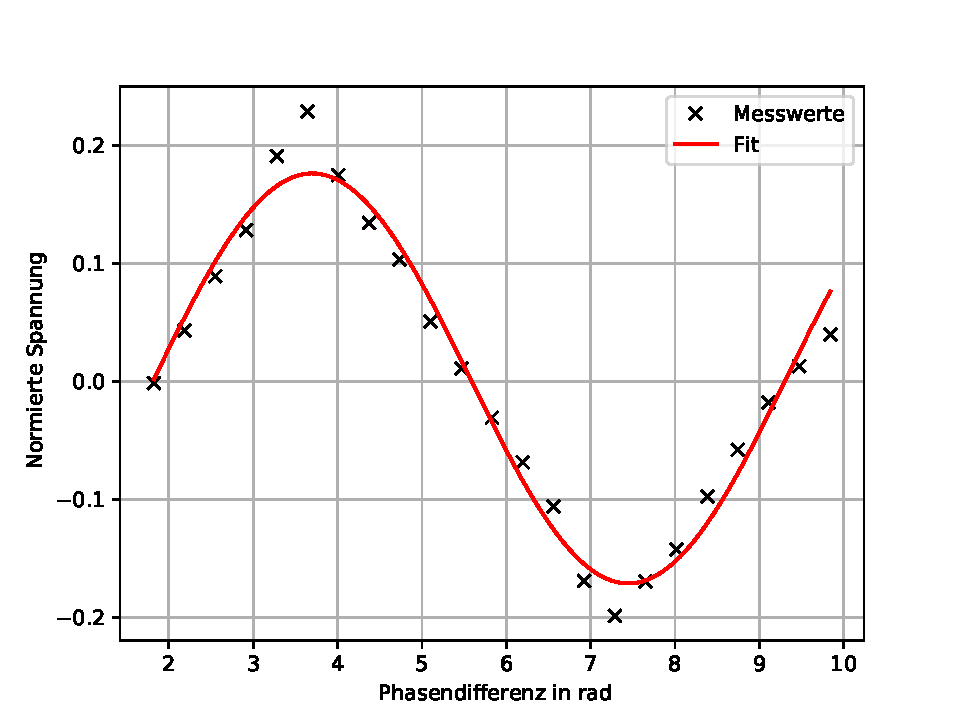
\includegraphics{build/plot.pdf}
%   \caption{Messdaten und Fitergebnis.}
%   \label{fig:plot}
% \end{figure}
%
% 2x2 Plot
% \begin{figure*}
%     \centering
%     \begin{subfigure}[b]{0.475\textwidth}
%         \centering
%         \includegraphics[width=\textwidth]{Abbildungen/Schaltung1.pdf}
%         \caption[]%
%         {{\small Schaltung 1.}}
%         \label{fig:Schaltung1}
%     \end{subfigure}
%     \hfill
%     \begin{subfigure}[b]{0.475\textwidth}
%         \centering
%         \includegraphics[width=\textwidth]{Abbildungen/Schaltung2.pdf}
%         \caption[]%
%         {{\small Schaltung 2.}}
%         \label{fig:Schaltung2}
%     \end{subfigure}
%     \vskip\baselineskip
%     \begin{subfigure}[b]{0.475\textwidth}
%         \centering
%         \includegraphics[width=\textwidth]{Abbildungen/Schaltung4.pdf}    % Zahlen vertauscht ... -.-
%         \caption[]%
%         {{\small Schaltung 3.}}
%         \label{fig:Schaltung3}
%     \end{subfigure}
%     \quad
%     \begin{subfigure}[b]{0.475\textwidth}
%         \centering
%         \includegraphics[width=\textwidth]{Abbildungen/Schaltung3.pdf}
%         \caption[]%
%         {{\small Schaltung 4.}}
%         \label{fig:Schaltung4}
%     \end{subfigure}
%     \caption[]
%     {Ersatzschaltbilder der verschiedenen Teilaufgaben.}
%     \label{fig:Schaltungen}
% \end{figure*}
